\documentclass{standalone}
\usepackage{tikz}
\usetikzlibrary{patterns, positioning}


\begin{document}
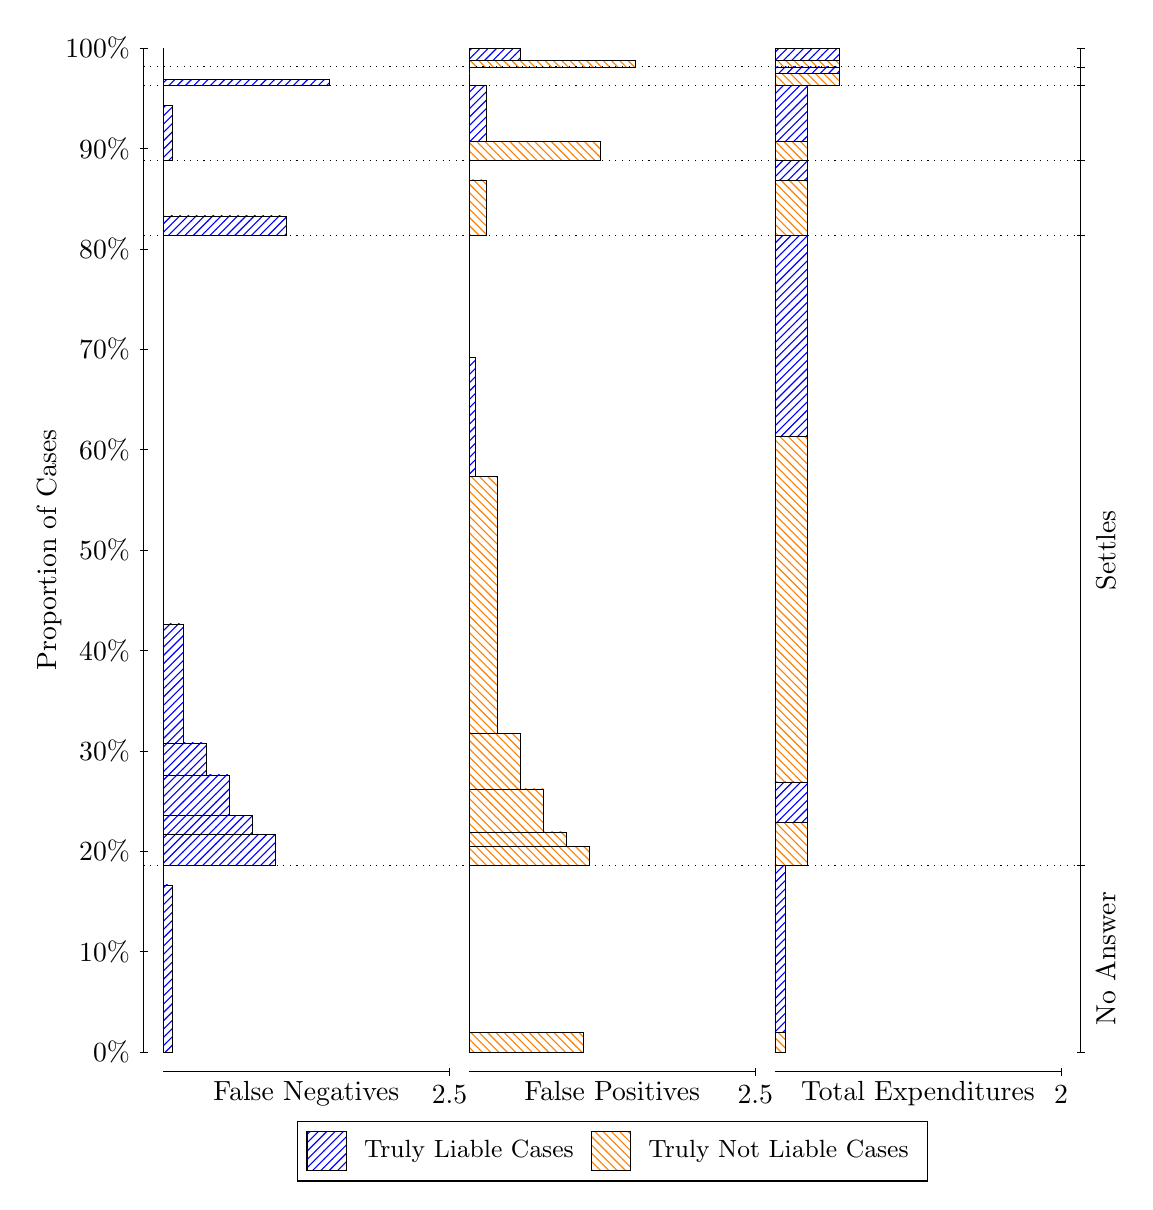
\begin{tikzpicture}
\draw[black, very thin] (1.5,1.75) -- (1.5,14.5);
\node[rotate=90, text=black, anchor=center] at (0.3, 8.125) {Proportion of Cases};
\draw[black, very thin] (1.45,1.75) -- (1.55,1.75);
\node[text=black, anchor=east] at (1.45, 1.75) {0\%};
\draw[black, very thin] (1.45,3.025) -- (1.55,3.025);
\node[text=black, anchor=east] at (1.45, 3.025) {10\%};
\draw[black, very thin] (1.45,4.3) -- (1.55,4.3);
\node[text=black, anchor=east] at (1.45, 4.3) {20\%};
\draw[black, very thin] (1.45,5.575) -- (1.55,5.575);
\node[text=black, anchor=east] at (1.45, 5.575) {30\%};
\draw[black, very thin] (1.45,6.85) -- (1.55,6.85);
\node[text=black, anchor=east] at (1.45, 6.85) {40\%};
\draw[black, very thin] (1.45,8.125) -- (1.55,8.125);
\node[text=black, anchor=east] at (1.45, 8.125) {50\%};
\draw[black, very thin] (1.45,9.4) -- (1.55,9.4);
\node[text=black, anchor=east] at (1.45, 9.4) {60\%};
\draw[black, very thin] (1.45,10.675) -- (1.55,10.675);
\node[text=black, anchor=east] at (1.45, 10.675) {70\%};
\draw[black, very thin] (1.45,11.95) -- (1.55,11.95);
\node[text=black, anchor=east] at (1.45, 11.95) {80\%};
\draw[black, very thin] (1.45,13.225) -- (1.55,13.225);
\node[text=black, anchor=east] at (1.45, 13.225) {90\%};
\draw[black, very thin] (1.45,14.5) -- (1.55,14.5);
\node[text=black, anchor=east] at (1.45, 14.5) {100\%};

\draw[black, very thin] (13.4,1.75) -- (13.4,14.5);
\draw[black, very thin] (13.35,1.75) -- (13.45,1.75);
\node[anchor=west] at (13.35, 1.75) {};
\draw[black, very thin] (13.35,4.1222) -- (13.45,4.1222);
\node[anchor=west] at (13.35, 4.1222) {};
\draw[black, very thin] (13.35,12.123) -- (13.45,12.123);
\node[anchor=west] at (13.35, 12.123) {};
\draw[black, very thin] (13.35,13.072) -- (13.45,13.072);
\node[anchor=west] at (13.35, 13.072) {};
\draw[black, very thin] (13.35,14.022) -- (13.45,14.022);
\node[anchor=west] at (13.35, 14.022) {};
\draw[black, very thin] (13.35,14.261) -- (13.45,14.261);
\node[anchor=west] at (13.35, 14.261) {};
\draw[black, very thin] (13.35,14.5) -- (13.45,14.5);
\node[anchor=west] at (13.35, 14.5) {};

\draw[black, very thin, pattern color=blue, pattern=north east lines] (1.75,1.75) rectangle (1.859,3.8726);
\draw[black, very thin, pattern color=orange, pattern=north west lines] (1.75,3.8726) rectangle (1.75,4.1222);
\draw[black, very thin, pattern color=blue, pattern=north east lines] (1.75,4.1222) rectangle (3.167,4.511);
\draw[black, very thin, pattern color=blue, pattern=north east lines] (1.75,4.511) rectangle (2.8763,4.7575);
\draw[black, very thin, pattern color=blue, pattern=north east lines] (1.75,4.7575) rectangle (2.5857,5.2692);
\draw[black, very thin, pattern color=blue, pattern=north east lines] (1.75,5.2692) rectangle (2.295,5.6765);
\draw[black, very thin, pattern color=blue, pattern=north east lines] (1.75,5.6765) rectangle (2.0043,7.1859);
\draw[black, very thin, pattern color=orange, pattern=north west lines] (1.75,7.1859) rectangle (1.75,12.123);
\draw[black, very thin, pattern color=blue, pattern=north east lines] (1.75,12.123) rectangle (3.3123,12.369);
\draw[black, very thin, pattern color=orange, pattern=north west lines] (1.75,12.369) rectangle (1.75,13.072);
\draw[black, very thin, pattern color=blue, pattern=north east lines] (1.75,13.072) rectangle (1.859,13.775);
\draw[black, very thin, pattern color=orange, pattern=north west lines] (1.75,13.775) rectangle (1.75,14.022);
\draw[black, very thin, pattern color=blue, pattern=north east lines] (1.75,14.022) rectangle (3.8573,14.106);
\draw[black, very thin, pattern color=orange, pattern=north west lines] (1.75,14.106) rectangle (1.75,14.261);
\draw[black, very thin, pattern color=orange, pattern=north west lines] (1.75,14.261) rectangle (1.75,14.345);
\draw[black, very thin, pattern color=blue, pattern=north east lines] (1.75,14.345) rectangle (1.75,14.5);
\draw[black, very thin, pattern color=orange, pattern=north west lines] (5.6333,1.75) rectangle (7.0867,1.9996);
\draw[black, very thin, pattern color=blue, pattern=north east lines] (5.6333,1.9996) rectangle (5.6333,4.1222);
\draw[black, very thin, pattern color=orange, pattern=north west lines] (5.6333,4.1222) rectangle (7.1593,4.3611);
\draw[black, very thin, pattern color=orange, pattern=north west lines] (5.6333,4.3611) rectangle (6.8687,4.5455);
\draw[black, very thin, pattern color=orange, pattern=north west lines] (5.6333,4.5455) rectangle (6.578,5.0924);
\draw[black, very thin, pattern color=orange, pattern=north west lines] (5.6333,5.0924) rectangle (6.2873,5.7953);
\draw[black, very thin, pattern color=orange, pattern=north west lines] (5.6333,5.7953) rectangle (5.9967,9.0591);
\draw[black, very thin, pattern color=blue, pattern=north east lines] (5.6333,9.0591) rectangle (5.706,10.569);
\draw[black, very thin, pattern color=blue, pattern=north east lines] (5.6333,10.569) rectangle (5.6333,12.123);
\draw[black, very thin, pattern color=orange, pattern=north west lines] (5.6333,12.123) rectangle (5.8513,12.826);
\draw[black, very thin, pattern color=blue, pattern=north east lines] (5.6333,12.826) rectangle (5.6333,13.072);
\draw[black, very thin, pattern color=orange, pattern=north west lines] (5.6333,13.072) rectangle (7.3047,13.319);
\draw[black, very thin, pattern color=blue, pattern=north east lines] (5.6333,13.319) rectangle (5.8513,14.022);
\draw[black, very thin, pattern color=orange, pattern=north west lines] (5.6333,14.022) rectangle (5.6333,14.176);
\draw[black, very thin, pattern color=blue, pattern=north east lines] (5.6333,14.176) rectangle (5.6333,14.261);
\draw[black, very thin, pattern color=orange, pattern=north west lines] (5.6333,14.261) rectangle (7.7407,14.345);
\draw[black, very thin, pattern color=blue, pattern=north east lines] (5.6333,14.345) rectangle (6.2873,14.5);
\draw[black, very thin, pattern color=orange, pattern=north west lines] (9.5167,1.75) rectangle (9.6529,1.9996);
\draw[black, very thin, pattern color=blue, pattern=north east lines] (9.5167,1.9996) rectangle (9.6529,4.1222);
\draw[black, very thin, pattern color=orange, pattern=north west lines] (9.5167,4.1222) rectangle (9.9254,4.6691);
\draw[black, very thin, pattern color=blue, pattern=north east lines] (9.5167,4.6691) rectangle (9.9254,5.1809);
\draw[black, very thin, pattern color=orange, pattern=north west lines] (9.5167,5.1809) rectangle (9.9254,9.5709);
\draw[black, very thin, pattern color=blue, pattern=north east lines] (9.5167,9.5709) rectangle (9.9254,12.123);
\draw[black, very thin, pattern color=orange, pattern=north west lines] (9.5167,12.123) rectangle (9.9254,12.826);
\draw[black, very thin, pattern color=blue, pattern=north east lines] (9.5167,12.826) rectangle (9.9254,13.072);
\draw[black, very thin, pattern color=orange, pattern=north west lines] (9.5167,13.072) rectangle (9.9254,13.319);
\draw[black, very thin, pattern color=blue, pattern=north east lines] (9.5167,13.319) rectangle (9.9254,14.022);
\draw[black, very thin, pattern color=orange, pattern=north west lines] (9.5167,14.022) rectangle (10.334,14.176);
\draw[black, very thin, pattern color=blue, pattern=north east lines] (9.5167,14.176) rectangle (10.334,14.261);
\draw[black, very thin, pattern color=orange, pattern=north west lines] (9.5167,14.261) rectangle (10.334,14.345);
\draw[black, very thin, pattern color=blue, pattern=north east lines] (9.5167,14.345) rectangle (10.334,14.5);
\draw[black, dotted] (1.5,4.1222) -- (13.4,4.1222);
\draw[black, dotted] (1.5,12.123) -- (13.4,12.123);
\draw[black, dotted] (1.5,13.072) -- (13.4,13.072);
\draw[black, dotted] (1.5,14.022) -- (13.4,14.022);
\draw[black, dotted] (1.5,14.261) -- (13.4,14.261);
\draw[black, very thin] (1.75,1.5) -- (5.3833,1.5);
\node[text=black, anchor=north] at (3.5667, 1.5) {False Negatives};
\draw[black, very thin] (5.3833,1.45) -- (5.3833,1.55);
\node[text=black, anchor=north] at (5.3833, 1.45) {2.5};

\draw[black, very thin] (5.6333,1.5) -- (9.2667,1.5);
\node[text=black, anchor=north] at (7.45, 1.5) {False Positives};
\draw[black, very thin] (9.2667,1.45) -- (9.2667,1.55);
\node[text=black, anchor=north] at (9.2667, 1.45) {2.5};

\draw[black, very thin] (9.5167,1.5) -- (13.15,1.5);
\node[text=black, anchor=north] at (11.333, 1.5) {Total Expenditures};
\draw[black, very thin] (13.15,1.45) -- (13.15,1.55);
\node[text=black, anchor=north] at (13.15, 1.45) {2};

\node[text=black, centered, rotate=90] at (13.72, 2.9361) {No Answer};
\node[text=black, centered, rotate=90] at (13.72, 8.1225) {Settles};





\draw (7.449999999999999,1.5) node[draw=none] (baseCoordinate) {};
\begin{scope}[align=center]
        \matrix[scale=0.5, draw=black, below=0.5cm of baseCoordinate, nodes={draw}, column sep=0.1cm]{
            \node[rectangle, draw, minimum width=0.5cm, minimum height=0.5cm, pattern color=blue, pattern=north east lines] {}; &
            \node[draw=none, font=\small, text=black] (B) {Truly Liable Cases}; &
            \node[rectangle, draw, minimum width=0.5cm, minimum height=0.5cm, pattern color=orange, pattern=north west lines] {}; &
            \node[draw=none, font=\small, text=black] (B) {Truly Not Liable Cases}; \\
            };
\end{scope}

\end{tikzpicture}
\end{document}